\tikzset{
    point/.style={
        thick,
        draw=gray,
        cross out,
        inner sep=0pt,
        minimum width=4pt,
        minimum height=4pt,
    },
}
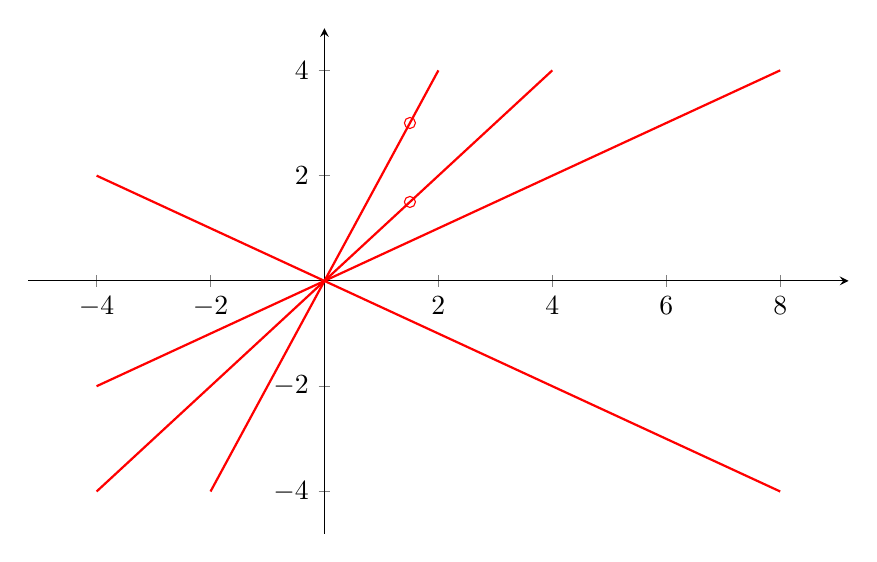
\begin{tikzpicture}
    \begin{axis}[
    legend pos=south east,
        axis x line=middle,
        axis y line=middle,
        %grid = major,
        width=12cm,
        height=8cm,
        %grid style={dashed, gray!30},
        xmin=-4,     % start the diagram at this x-coordinate
        xmax= 8,    % end   the diagram at this x-coordinate
        ymin=-4,     % start the diagram at this y-coordinate
        ymax= 4,   % end   the diagram at this y-coordinate
        axis background/.style={fill=white},
        %xticklabels={-2,-1.6,...,2},
        %yticklabels={-8,-7,...,8},
        %tick align=outside,
        enlargelimits=true,
        tension=0.08]
      % plot the stirling-formulae
      \addplot[domain=-4:8, red, thick,samples=500] {0.5*x}; 
      \addplot[domain=-2:2, red, thick,samples=500] {2*x}; 
      \addplot[domain=-4:4, red, thick,samples=500] {x}; 
      \addplot[domain=-4:8, red, thick,samples=500] {-0.5*x}; 
      \addplot[color=red,only marks,mark=o]
        plot coordinates {
            (1.5,3)
            (1.5,1.5)
        };
    \end{axis} 
\end{tikzpicture}
